\documentclass[11pt,a4paper]{article}

\usepackage[utf8]{inputenc}
\usepackage[T1]{fontenc}
\usepackage{lmodern}
\usepackage[margin=2.4cm]{geometry}
\usepackage{amsmath,amssymb}
\usepackage{physics}
\usepackage{graphicx}
\usepackage{booktabs}
\usepackage{microtype}
\usepackage{hyperref}
\usepackage{listings}
\usepackage{xcolor}
\usepackage{caption}
\usepackage{float}
\usepackage{parskip}

\hypersetup{colorlinks=true,linkcolor=blue,citecolor=blue,urlcolor=blue}

\captionsetup{font=small, labelfont=bf, width=0.95\textwidth}

\lstset{
  language=Python,
  basicstyle=\ttfamily\small,
  keywordstyle=\color{blue!70!black},
  commentstyle=\color{gray},
  stringstyle=\color{orange!80!black},
  numbers=none,
  frame=single,
  framerule=0.5pt,
  rulecolor=\color{black!20},
  backgroundcolor=\color{black!3},
  breaklines=false,
  keepspaces=true,
  showstringspaces=false,
  xleftmargin=6pt,
  xrightmargin=6pt,
}

\title{\textbf{Dynamical Phase Transitions in the Transverse-Field Ising Model\\
via Infinite Time-Evolving Block Decimation}\\[4pt]
\large TNS/DMRG Course, Project A4, BME Spring 2026}
\author{P\'eter Tall\'osy \quad \texttt{K14WR1}}
\date{}

\begin{document}
\maketitle
\vspace{-8pt}

% ============================================================
\begin{abstract}
Quantum quenches in the infinite one-dimensional transverse-field Ising model
(TFIM) are simulated using iTEBD, starting from the antiferromagnetic Neel
state. The Loschmidt rate function $\lambda(t)$ develops non-analytic cusps
(dynamical phase transitions, DPTs) when the post-quench field $h$
exceeds the quantum critical value $h=1$. Cusp positions are characterized as
a function of $h$, order-parameter dynamics are analyzed, and a systematic
error budget is performed, showing that Trotter discretization ($\delta t = 0.05$) dominates
over bond-dimension truncation by six orders of magnitude, a direct consequence
of the TFIM's free-fermion integrability. An extended run to $t=15$ resolves
an ambiguous feature at $h=0.8$ as a genuine DPT, indicating that the DPT
threshold for the Neel initial state lies below the equilibrium critical field
$h=1$. All simulations are performed directly in the thermodynamic limit,
avoiding finite-size effects entirely.
\end{abstract}

% ============================================================
\section{Introduction}
\label{sec:intro}
% ============================================================

A quantum quench is the sudden, instantaneous change of a Hamiltonian
parameter at $t=0$: the system is prepared in some initial state $|\psi_0\rangle$
and then evolves under a new, post-quench Hamiltonian for all $t>0$. This
drives the system out of equilibrium and builds up correlations over time. A striking
phenomenon that can arise is the dynamical phase transition (DPT)
\cite{heyl2013}, characterized by non-analytic cusps in the Loschmidt rate
function $\lambda(t) = -\ln|G(t)|$, where $G(t) = \bra{\psi_0}e^{-iHt}\ket{\psi_0}$
is the Loschmidt echo. These cusps are the dynamical analogue of equilibrium
phase transitions: just as the free energy density is non-analytic at a
critical temperature, $\lambda(t)$ is non-analytic at critical times $t^*_n$
when $G(t^*_n) = 0$ exactly in the thermodynamic limit.

This is studied in the one-dimensional TFIM using the infinite time-evolving
block decimation (iTEBD) algorithm \cite{vidal2007}, which represents the
quantum state as an infinite matrix product state (MPS) and evolves it via
Suzuki--Trotter decomposition \cite{suzuki1976,hatano2005}. Working directly on the
infinite chain eliminates finite-size effects, and the Loschmidt echo is
extracted as the dominant eigenvalue of a single transfer matrix; no
finite-size extrapolation is needed. The reference implementation follows the
MATLAB code provided in the course notes; this project reimplements and extends
it in Python with NumPy and SciPy.

% ============================================================
\section{Model and Setup}
\label{sec:model}
% ============================================================

The TFIM Hamiltonian on an infinite chain is
\begin{equation}
  H(h) = -J\sum_{i} Z_i Z_{i+1} - h\sum_{i} X_i,
  \label{eq:tfim}
\end{equation}
with $J=1$ throughout. The $ZZ$ term favors ferromagnetic alignment; the
transverse field $X$ flips individual spins and drives the system toward a
paramagnetic state. These two tendencies compete, producing an exact quantum
phase transition (QPT) at $h=1$ \cite{sachdev2011}. The model is exactly
solvable: the Jordan--Wigner transformation $c_j = \bigl(\prod_{k<j}Z_k\bigr)\sigma^-_j$
maps it to a quadratic (free-fermion) Hamiltonian, exactly diagonalized
in momentum space by a Bogoliubov transformation (a rotation that mixes
particle operators $c_k$ and $c_{-k}^\dagger$ into independent quasiparticle
modes with dispersion $\varepsilon_k(h)$, eliminating all interaction terms).

The system is initialized in the Neel state $\ket{\psi_0} = \ket{\uparrow\downarrow\uparrow\downarrow\cdots}$
and evolved under $H(h)$:
\begin{equation}
  \ket{\psi(t)} = e^{-iH(h)t}\ket{\psi_0}.
\end{equation}
The Neel state is chosen not because it is an equilibrium state (it is not
the ground state of any $h\geq 0$ in the ferromagnetic TFIM), but because it
is the unique product state ($\chi=1$ MPS) compatible with the two-sublattice
unit cell that iTEBD requires, and it provides a well-defined non-trivial
initial condition for studying DPT dynamics.

% ============================================================
\section{Method}
\label{sec:method}
% ============================================================

\subsection{Why the Hilbert space can be compressed}

\textbf{Reduced density matrices.} For a pure state $\ket{\psi}$, the density
matrix is simply $\rho = \ket{\psi}\bra{\psi}$: a complete description of the
state, equivalent to $\ket{\psi}$ itself. Cutting the chain into a left half
$L$ and a right half $R$, the reduced density matrix of the left half is
obtained by tracing out (summing over) every right-half degree of freedom,
\begin{equation}
  \rho_L = \mathrm{Tr}_R\, \rho = \mathrm{Tr}_R\, \ket{\psi}\bra{\psi}.
\end{equation}
$\rho_L$ is what an observer with access to only the left half would measure:
it answers every question about the left subsystem alone, with the right
subsystem averaged over. Inserting the Schmidt decomposition,
Eq.~\eqref{eq:schmidt}, the trace over $R$ collapses onto the orthonormal
$\ket{v_\alpha}_R$ states, giving
\begin{equation}
  \rho_L = \sum_{\alpha=0}^{\chi-1} \lambda_\alpha^2\, \ket{u_\alpha}_L\bra{u_\alpha}_L.
  \label{eq:rho_L}
\end{equation}
This is already diagonal: the Schmidt vectors $\ket{u_\alpha}_L$ are exactly
the eigenvectors of $\rho_L$, with eigenvalues $\lambda_\alpha^2 \geq 0$
summing to 1 (probabilities). The \emph{rank} of $\rho_L$, the number of
nonzero eigenvalues, is precisely $\chi$. $\chi$ is the number of
distinguishable outcomes a measurement on the left half alone could ever
produce, given everything the right half could be
correlated with. A product state has $\rho_L$ pure (rank 1, $\chi=1$): the
left half is in a definite state regardless of the right half. The von
Neumann entanglement entropy used throughout this report,
$S_L = -\mathrm{Tr}\,\rho_L \ln \rho_L = -\sum_\alpha \lambda_\alpha^2 \ln
\lambda_\alpha^2$, is the Shannon entropy of this eigenvalue distribution: it
is zero exactly when $\chi=1$, and grows with $\chi$ and with how evenly the
weight $\lambda_\alpha^2$ is spread across the $\chi$ Schmidt modes.

\textbf{What $\chi$ represents physically.} On the 1D lattice, $\chi$ at a
given bond is the number of independent channels through which the left half
and the right half can be correlated at that bond. A classical analogy: if a
cable between two halves of a circuit carries $\chi$ independent wires,
$\chi=1$ means the two sides can only ever agree on one shared value (no real
information flows), while large $\chi$ allows many simultaneous, independent
correlations. Entanglement entropy is bounded by the channel count,
$S_L \leq \ln \chi$, with equality when all $\chi$ Schmidt weights are equal
($\lambda_\alpha^2 = 1/\chi$ for all $\alpha$, the maximally mixed case).
Equivalently, representing a state with entanglement entropy $S_L$ requires
at least $\chi \geq e^{S_L}$ Schmidt modes. This inequality is the precise
link between the physics of entanglement and the cost of the MPS
representation below: bounding $S_L$ bounds the minimum $\chi$ needed.

Compression to small $\chi$ is possible because of two physical facts about
$S_L$, not because we choose to throw information away. First, ground states
of gapped, local Hamiltonians obey an area law: $S_\ell = O(1)$ for a
bipartition at site $\ell$, a constant independent of the subsystem size
$\ell$ (or $L-\ell$), as opposed to a volume law $S_\ell \sim \alpha\min(\ell,
L-\ell)$, which is what a generic (Haar-random) state has, and which would
require $\chi \sim e^{\alpha \ell}$, exponential in system size. Second, for
the \emph{dynamics} studied here, the Lieb-Robinson bound limits how fast
$S_\ell(t)$ can grow after a quench from a low-entanglement initial state:
information and correlations travel at a finite effective speed $v_{\rm LR}$,
giving $S_\ell(t) \lesssim v_{\rm LR}\, t$ (linear in time) rather than an
instantaneous jump to the volume-law maximum. Both facts mean $\chi \geq
e^{S_\ell(t)}$ stays small, or grows at most as $e^{v_{\rm LR} t}$ over the
finite simulation window, for the states that actually appear in this
simulation, even though $\chi$ could in principle be as large as
$2^{\min(L,\,L-\ell)}$ for an arbitrary state. This is the entire reason MPS
methods work at all: they are a general-purpose tool that happens to be very
efficient on the particular, low-entanglement corner of Hilbert space that
physical time evolution actually explores.

There is a second compression at work, specific to this project: translation
invariance. The chain is infinite, so representing it site by site is
impossible regardless of $\chi$. The Neel initial state $\ket{\uparrow
\downarrow \uparrow \downarrow \cdots}$ is invariant under translation by two
sites (not one), so the converged state retains this two-site periodicity for
all time. As a result, a single pair of tensors per sublattice, repeated
forever, describes the full infinite chain exactly: this is what makes
$(\Gamma^A,\Lambda^A,\Gamma^B,\Lambda^B)$ sufficient data for an infinite
system. No further symmetry is exploited in the code: the TFIM also has a
global $\mathbb{Z}_2$ (spin-flip) symmetry generated by $P = \prod_i X_i$,
which commutes with $H$, but the tensors here are not decomposed into
symmetry sectors. Implementing $\mathbb{Z}_2$-symmetric tensors would reduce
memory and let $\chi_{\max}$ be pushed higher at fixed cost, but is not needed
at the bond dimensions used in this work (Section~\ref{sec:results} shows
$\chi_{\max}=40$ is already far above what is required for convergence).

\subsection{MPS and the Vidal canonical form}

For low-entanglement states, the saving above is realized concretely by
writing the state as a matrix product state (MPS). At any bipartition of the
chain into left ($L$) and right ($R$) halves, the Schmidt decomposition gives
\begin{equation}
  \ket{\psi} = \sum_{\alpha=0}^{\chi-1} \lambda_\alpha \ket{u_\alpha}_L \ket{v_\alpha}_R,
  \label{eq:schmidt}
\end{equation}
where $\lambda_\alpha$ are the Schmidt values, ordered by magnitude. The bond
dimension $\chi$ counts the number of terms: $\chi=1$ is a product state (zero
entanglement), and larger $\chi$ encodes more entanglement. $\chi$ is a
property of the quantum state itself at each moment in time: as
entanglement builds up during evolution, $\chi$ grows. For a generic state
after a long quench, $\chi$ would need to grow exponentially, making simulation
infeasible. The practical solution is to impose a cap $\chi_{\max}$: keep only
the $\chi_{\max}$ largest Schmidt values and discard the rest. When the true
$\chi$ of the state is below $\chi_{\max}$, the MPS is exact. When it
exceeds $\chi_{\max}$, the simulation becomes approximate, with error
$\varepsilon_{\rm trunc} = \sum_{\alpha \geq \chi_{\max}} \lambda_\alpha^2$.
The bond dimension $\chi_{\max}$ is therefore both the precision knob and the
memory cost of the simulation.

An MPS expresses the full state as a chain of local matrices, one per site:
\begin{equation}
  \ket{\psi} = \sum_{s_1,\dots,s_L} A^{[1]s_1} A^{[2]s_2} \cdots A^{[L]s_L}
  \ket{s_1 s_2 \cdots s_L},
\end{equation}
where each $A^{[i]s_i}$ is a $\chi\times\chi$ matrix with physical index
$s_i \in \{\uparrow,\downarrow\}$. Memory scales as $d\chi^2 L$ instead of
$d^L$, making simulation efficient as long as $\chi$ stays bounded.

Each time a two-site gate is applied, the bond dimension across that bond can
double. The compression step that keeps it bounded is a \textbf{singular value
decomposition (SVD)}: after contracting a two-site block into a $(d\chi)\times(d\chi)$
matrix $M$, factorize $M = U S V^\dagger$, where the diagonal of $S$ holds
the singular values $\lambda_0 \geq \lambda_1 \geq \cdots$ in descending order.
Retaining only the $\chi_{\max}$ largest and discarding the rest brings the bond
back to $\chi_{\max}$. This truncation is optimal by Schmidt's theorem: no
rank-$\chi_{\max}$ approximation achieves a smaller error than
$\varepsilon_{\rm trunc} = \sum_{\alpha\geq\chi_{\max}}\lambda_\alpha^2$.
The singular values from the SVD are precisely the Schmidt values $\lambda_\alpha$
in Eq.~\eqref{eq:schmidt}, so the two pictures (Schmidt decomposition and
SVD-based MPS compression) are the same operation viewed from different angles.

For this system, the Vidal canonical form \cite{vidal2007} uses four objects
$(\Gamma^A, \Lambda^A, \Gamma^B, \Lambda^B)$ that tile the infinite chain as
\begin{equation*}
  \cdots\, \Lambda^B_\alpha\;\Gamma^A_{\alpha\gamma}[s_A]\;\Lambda^A_\gamma\;
  \Gamma^B_{\gamma\beta}[s_B]\;\Lambda^B_\beta \,\cdots
\end{equation*}
Four tensors are required because the Neel state has a two-site period: A-sites
(even, initial spin $\uparrow$) and B-sites (odd, initial spin $\downarrow$) evolve
differently, so $\Gamma^A \neq \Gamma^B$ throughout.

\textbf{What $\Lambda$ is.} Each $\Lambda$ is simply a 1D array (vector) of
$\chi$ non-negative real numbers, ordered from largest to smallest:
$\Lambda^A_0 \geq \Lambda^A_1 \geq \cdots \geq 0$.
These are exactly the Schmidt values at the bond (the singular values produced
by SVD, as in Eq.~\eqref{eq:schmidt}). $\Lambda^A_\gamma$ gives the weight of
the $\gamma$-th Schmidt mode at the A-bond; $\Lambda^B_\alpha$ does the same at
B-bonds. There is nothing more to them than that.

\textbf{What $\Gamma$ is.} Each $\Gamma$ is a 3-index array of numbers (a rank-3
tensor). $\Gamma^A$ has shape $\chi_B \times 2 \times \chi_A$: three indices
covering all combinations of left Schmidt state $\alpha$, spin $s \in
\{\uparrow,\downarrow\}$, and right Schmidt state $\gamma$. The number
$\Gamma^A_{\alpha, s, \gamma}$ is a coefficient: it says how much amplitude
the state carries when site A has spin $s$, the entanglement mode on its left
is $\alpha$, and the entanglement mode on its right is $\gamma$. Fixing the spin
index gives a $\chi_B \times \chi_A$ matrix that rotates between the Schmidt
basis on the left bond and the Schmidt basis on the right bond. The $\Gamma$
tensor encodes geometry and connectivity; the actual amplitude weights live
in $\Lambda$. This is why the transfer matrix uses ``dressed'' tensors
(Section~\ref{sec:transfer}): $\Gamma$ alone is incomplete without $\Lambda$.

The von Neumann entropy $S_A = -\sum_\gamma (\Lambda^A_\gamma)^2
\ln(\Lambda^A_\gamma)^2$ is immediately readable from $\Lambda^A$.
At $t=0$ (Neel state), $\chi_A = \chi_B = 1$: all bond indices take a single
value and every tensor reduces to a single number.

\subsection{iTEBD: Trotter gates and Vidal update}

The TFIM Hamiltonian naturally splits as $H = H_{AB} + H_{BA}$, where $H_{AB}$
contains all nearest-neighbor bond terms between A-sites (even) and B-sites
(odd), and $H_{BA}$ contains the B-to-A bonds. Within each group, all terms
act on disjoint pairs of sites and commute, so $e^{-iH_{AB}\delta t} = \prod_k e^{-ih_{2k,2k+1}\delta t}$.
Between groups, however, $[H_{AB}, H_{BA}] \neq 0$, requiring a Trotter approximation.

The second-order (Strang) decomposition is used:
\begin{equation}
  e^{-iH\delta t} \approx e^{-iH_{AB}\delta t/2}\, e^{-iH_{BA}\delta t}\, e^{-iH_{AB}\delta t/2} + O(\delta t^3).
  \label{eq:trotter}
\end{equation}
The symmetric split cancels the first-order $[H_{AB}, H_{BA}]$ error exactly,
reducing the per-step error from $O(\delta t^2)$ to $O(\delta t^3)$ and the
global error from $O(\delta t)$ to $O(\delta t^2)$. This is why each full step
uses a \emph{half-step gate} $U_{AB}(\delta t/2)$ at both ends and a
\emph{full-step gate} $U_{BA}(\delta t)$ in the middle.

Applying each 2-site gate to the Vidal MPS follows a five-step local update
(absorb, contract, apply gate, SVD, restore). The SVD output is truncated to
$\chi_{\max}$ singular values; the discarded weight $\varepsilon_{\rm trunc} = \sum_{\alpha\geq\chi_{\max}} \lambda_\alpha^2$
is recorded at each step. A compact implementation in Python is:

\begin{minipage}{\linewidth}
\begin{lstlisting}
# absorb environment Schmidt values
T1 = np.einsum('a,sab,b->sab', lB, GA, lA)   # dressed A tensor
T2 = np.einsum('sbc,c->sbc', GB, lB_right)    # dressed B tensor
# contract into 2-site tensor, apply gate, SVD + truncate
Theta = np.tensordot(T1, T2, axes=([2],[1]))
Theta = np.einsum('ijkl,klmn->ijmn', gate, Theta.transpose(1,0,2,3))
M = Theta.reshape(d * chiL, d * chiR)
U, S, Vh = np.linalg.svd(M, full_matrices=False)
S, U, Vh = S[:chi_max], U[:, :chi_max], Vh[:chi_max, :]
# restore Vidal form (divide out environment)
GA_new = (U.reshape(d, chiL, -1) / lB[:, None])
GB_new = (Vh.reshape(-1, d, chiR) / lB_right[None, :]).transpose(1,0,2)
lA_new = S / np.linalg.norm(S)
\end{lstlisting}
\end{minipage}

\subsection{Transfer matrix and the Loschmidt rate function}
\label{sec:transfer}

For the Neel initial state (a product state with $\chi=1$), the Loschmidt
amplitude factorizes over unit cells:
\begin{equation}
  G(t) = \bra{\psi_0}\psi(t)\rangle = \tau(t)^{L/2},
\end{equation}
where $\tau(t)$ is the dominant eigenvalue of the transfer matrix $T$. The
per-site rate function is then
\begin{equation}
  \lambda(t) = -\lim_{L\to\infty}\frac{1}{L}\ln|G(t)|^2 = -\ln|\tau(t)|,
  \label{eq:lambda}
\end{equation}
and $L$ cancels exactly. To build $T$, define dressed tensors
$A(t)^\sigma_{\alpha\gamma} = \Lambda^B_\alpha\, \Gamma^A(t)^\sigma_{\alpha\gamma}\, \Lambda^A_\gamma$
and $B(t)^\sigma_{\gamma\beta} = \Gamma^B(t)^\sigma_{\gamma\beta}\, \Lambda^B_\beta$.
``Dressed'' means the neighboring $\Lambda$ vectors are multiplied into $\Gamma$:
the bare $\Gamma$ encodes the tensor geometry but not the amplitude weights,
so the $\Lambda$ factors must be absorbed before computing any overlap.
Then
\begin{equation}
  T[\alpha,\beta] = \sum_\gamma A(t)^\uparrow_{\alpha\gamma}\, B(t)^\downarrow_{\gamma\beta}.
  \label{eq:transfer}
\end{equation}
$A(t)$ absorbs Schmidt values from both its neighbors (three factors), while
$B(t)$ absorbs only its right neighbor (two factors), ensuring each $\Lambda$
appears exactly once in the infinite product. The spin projections $\uparrow$
(A-site) and $\downarrow$ (B-site) come from the Neel initial state.

\subsection{No finite-size effects}

The iTEBD algorithm stores only the four tensors $(\Gamma^A, \Lambda^A, \Gamma^B, \Lambda^B)$,
implicitly representing an infinite chain by tiling. Gates are applied
identically to every AB bond and every BA bond simultaneously; there are no
boundaries. Because $\lambda(t) = -\ln|\tau|$ follows directly from a $\chi_B \times \chi_B$
eigenproblem, no finite-$L$ simulation or extrapolation is ever needed. The
only approximations are the bond-dimension cap $\chi_{\max}$ and the Trotter
step $\delta t$.

% ============================================================
\section{Results}
\label{sec:results}
% ============================================================

\subsection{Dynamical phase transitions and cusp positions}

\begin{figure}[t]
  \centering
  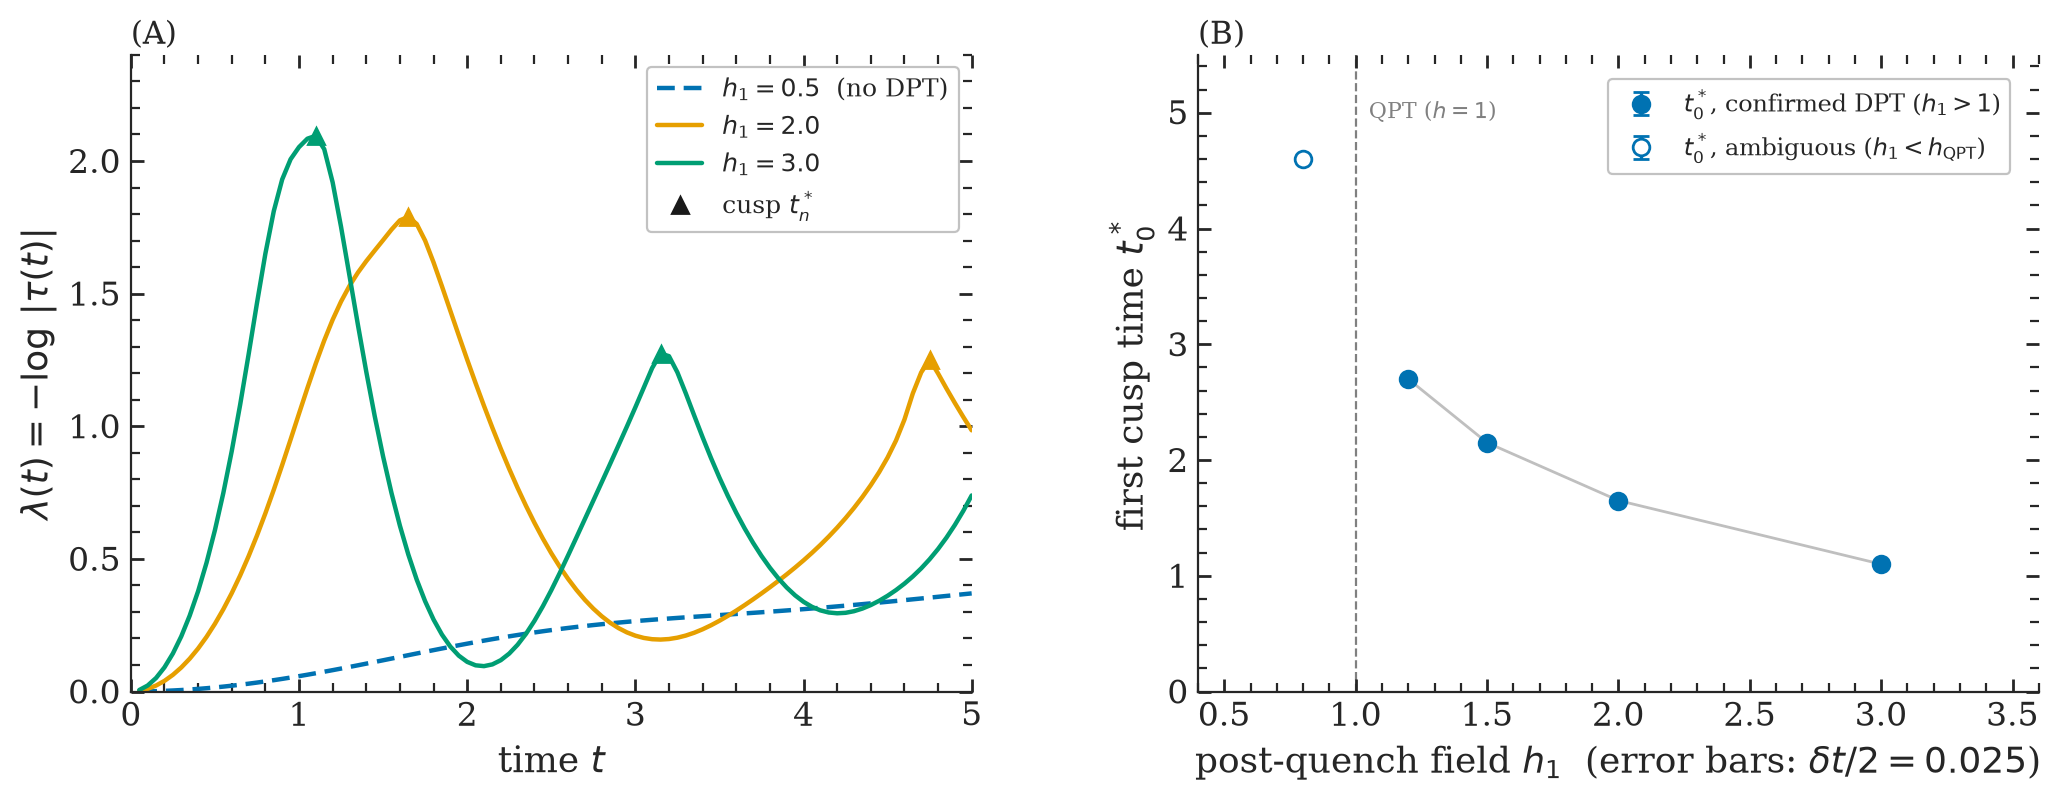
\includegraphics[width=\textwidth]{../results/figures/fig1_dpt_physics.png}
  \caption{\textbf{(A)} Loschmidt rate function $\lambda(t)$ for post-quench
    fields $h=0.5$, $2.0$, $3.0$. For $h<1$ (blue dashed), $\lambda(t)$ is
    smooth. For $h>1$ the rate function develops sharp peaks (cusps) at
    times $t^*_n$; in the exact theory $G(t^*_n)=0$ and $\lambda$ diverges,
    but finite $\chi_{\max}$ and $\delta t$ cap the peak at a finite value.
    Markers indicate detected cusp positions.
    \textbf{(B)} First cusp time $t^*_0$ as a function of $h$. Larger post-quench
    fields produce faster oscillations (larger quasi-particle energy). The open
    marker at $h=0.8$ is resolved as a genuine DPT by extended simulation (see
    Section~\ref{sec:h08}). Error bars reflect the Trotter step $\delta t = 0.025$.}
  \label{fig:dpt}
\end{figure}

Figure~\ref{fig:dpt}A shows $\lambda(t)$ for three representative post-quench
fields. At $h=0.5$ (quench within the ordered phase), $\lambda(t)$ grows
smoothly and never diverges: the Loschmidt echo $|G(t)|$ stays strictly
positive, meaning the time-evolved state $|\psi(t)\rangle$ never becomes
orthogonal to the initial Neel state. The quench is not energetically strong
enough to drive the system across a dynamical boundary.

At $h=2.0$ and $h=3.0$ (quench across the QPT at $h=1$), $\lambda(t)$
develops sharp, periodic peaks. In the exact (untruncated, continuous-time)
theory, $G(t^*_n) = 0$ at each cusp time and $\lambda(t^*_n)$ diverges:
quasi-particle excitations created by the quench interfere destructively at
intervals $\Delta t^* \propto 1/\varepsilon_{k^*}$, driving the Loschmidt
echo to zero. In the simulation, finite $\chi_{\max}$ and $\delta t$ prevent
an exact zero, so the peaks are finite; the first cusp of $h=2.0$ reaches
$\lambda \approx 1.79$. The non-analytic kink at each peak is the DPT
signature even in the approximate simulation.

For $h<1$, no zeros of $G(t)$ appear on the real time axis and $\lambda(t)$
is smooth throughout. The DPT is a thermodynamic-limit phenomenon: it is absent
from any finite system and emerges only as $L\to\infty$. The connection to
equilibrium phase transitions is direct: the zeros of $G(z)$ in the
complex-time plane are the dynamical analogue of Fisher zeros, and the DPT
occurs when those zeros cross the real axis.

Panel B shows the first cusp time $t^*_0$ as a function of post-quench field.
Larger $h$ drives faster quasi-particle dynamics (higher $\varepsilon_{k^*}$),
pulling $t^*_0$ to earlier times. The filled markers form a smooth curve for
$h > 1$; the open marker at $h = 0.8$ sits below the QPT and is discussed
in Section~\ref{sec:h08}.

The first cusp times from our simulation are:
\begin{center}
\small
\begin{tabular}{ccccc}
\toprule
$h$ & 1.2 & 1.5 & 2.0 & 3.0 \\
\midrule
$t^*_0$ & 2.70 & 2.15 & 1.65 & 1.10 \\
\bottomrule
\end{tabular}
\end{center}
The product $t^*_0 \cdot h$ is nearly constant across all simulated fields
($1.2 \times 2.70 = 3.24$, $1.5 \times 2.15 = 3.23$, $2.0 \times 1.65 = 3.30$,
$3.0 \times 1.10 = 3.30$), confirming $t^*_0 \propto 1/h$ empirically.
This is consistent with the quasi-particle picture $\Delta t^* \propto 1/\varepsilon_{k^*}$
when $\varepsilon_{k^*} \propto h$ for $h \gg J = 1$.
The cusp positions differ from the analytic result for the ferromagnetic
ground-state initial condition in Ref.~\cite{heyl2013} (which uses a different
initial state), but the qualitative physics is identical.

\subsection{Order parameter dynamics}

\begin{figure}[H]
  \centering
  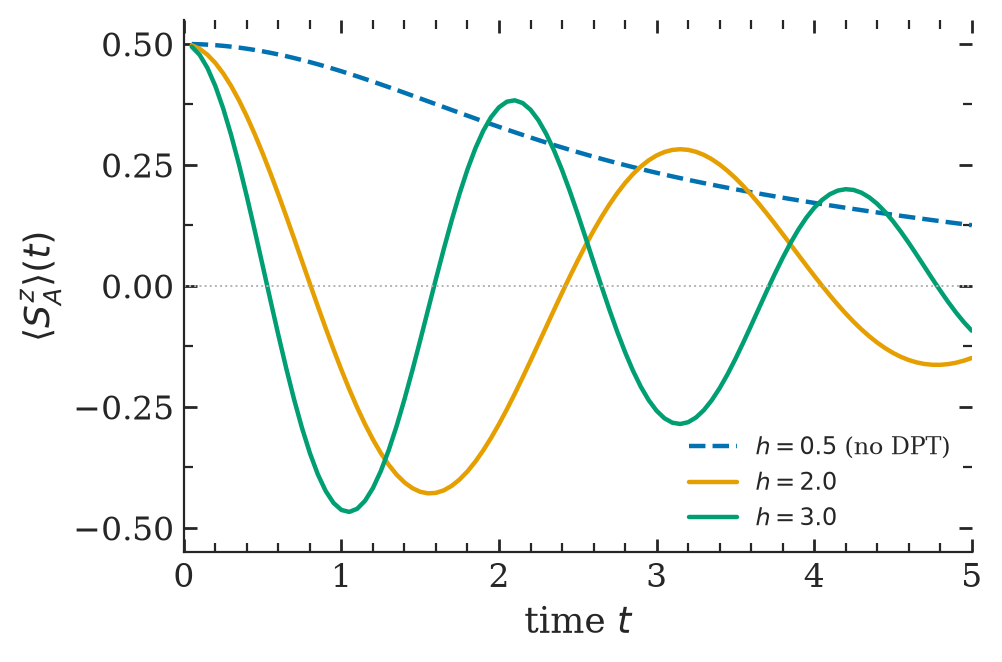
\includegraphics[width=0.72\textwidth]{../results/figures/fig4_order_parameter.png}
  \caption{A-sublattice magnetization $\langle S^z_A\rangle(t)$ for three
    post-quench fields. Starting from the Neel value $+1/2$, spins evolve
    under the transverse field. For $h=0.5$ (below QPT) the magnetization
    decays slowly and remains positive throughout, indicating the system stays
    near the ordered phase. For $h=2.0$ and $h=3.0$ (above QPT) the
    magnetization oscillates with increasing frequency and amplitude, reflecting
    the quasi-particle oscillations that also drive the DPT cusps in
    $\lambda(t)$.}
  \label{fig:sz}
\end{figure}

Figure~\ref{fig:sz} shows the A-sublattice magnetization $\langle S^z_A\rangle(t)$
complementing the $\lambda(t)$ picture. Below the QPT ($h=0.5$), spins precess
slowly while keeping positive average magnetization: the transverse field is
not strong enough to reverse the spin orientation. Above the QPT the
oscillation period decreases with $h$, consistent with the cusp period in
Figure~\ref{fig:dpt}. The $\langle S^z_A\rangle$ oscillations and the
$\lambda(t)$ cusps are driven by the same quasi-particle dynamics; the cusps
occur near the minima of $\langle S^z_A\rangle$, where the state is most
orthogonal to the initial Neel state.

\subsection{Bond dimension convergence and error budget}

\begin{figure}[H]
  \centering
  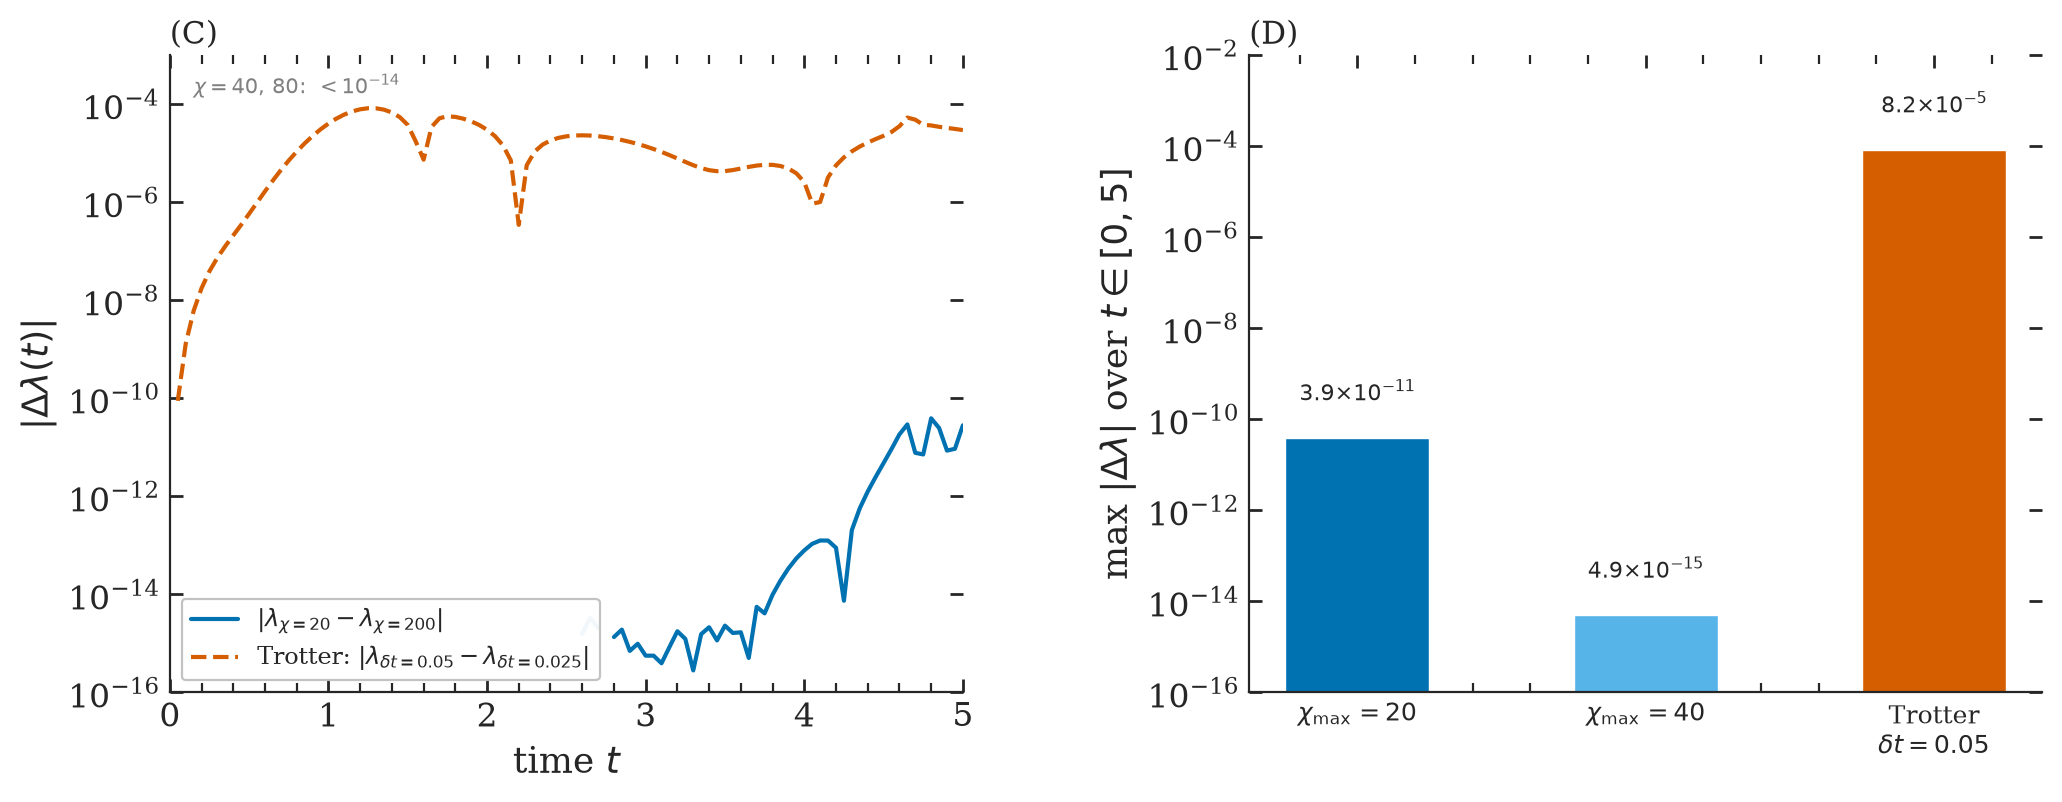
\includegraphics[width=\textwidth]{../results/figures/fig2_error_analysis.png}
  \caption{\textbf{(C)} Absolute error in $\lambda(t)$ comparing $\chi_{\max}=20$
    and $\chi_{\max}=200$ (blue), and comparing Trotter steps $\delta t = 0.05$
    and $\delta t = 0.025$ (orange dashed). The Trotter error dominates by many
    orders of magnitude. \textbf{(D)} Maximum error over $t\in[0,5]$ per error
    source. For $\chi_{\max}\geq 40$, chi-truncation error reaches machine precision;
    the simulation is entirely Trotter-limited.}
  \label{fig:error}
\end{figure}

Figure~\ref{fig:error} and the table below show the systematic error budget:
\begin{center}
\small
\begin{tabular}{lc}
\toprule
Source & $\max|\Delta\lambda|$ over $t\in[0,5]$ \\
\midrule
$\chi_{\max}=20$ vs $\chi_{\max}=200$ & $3.85\times10^{-11}$ \\
$\chi_{\max}=40$ vs $\chi_{\max}=200$ & $4.89\times10^{-15}$ \\
Trotter $\delta t=0.05$ vs $\delta t=0.025$ & $8.16\times10^{-5}$ \\
\bottomrule
\end{tabular}
\end{center}

The Trotter error exceeds bond-dimension truncation by six orders of magnitude.
This is a direct consequence of the TFIM's integrability: Jordan--Wigner
transformation maps the model to free fermions, which build entanglement only
logarithmically in time. At $t=5$ the actual bond dimension is $\chi_A = 53$,
well below $\chi_{\max}=200$, so very few Schmidt values are ever discarded.
The Trotter ratio $\delta t=0.1$ vs $\delta t=0.05$ gives error ratio $\approx 5$
(theory predicts $4$ for second-order Trotter), consistent within the
non-uniform error distribution near cusps. To improve accuracy, reducing
$\delta t$ is the only lever that matters here.

\subsection{Entanglement growth and bond dimension saturation}

\begin{figure}[H]
  \centering
  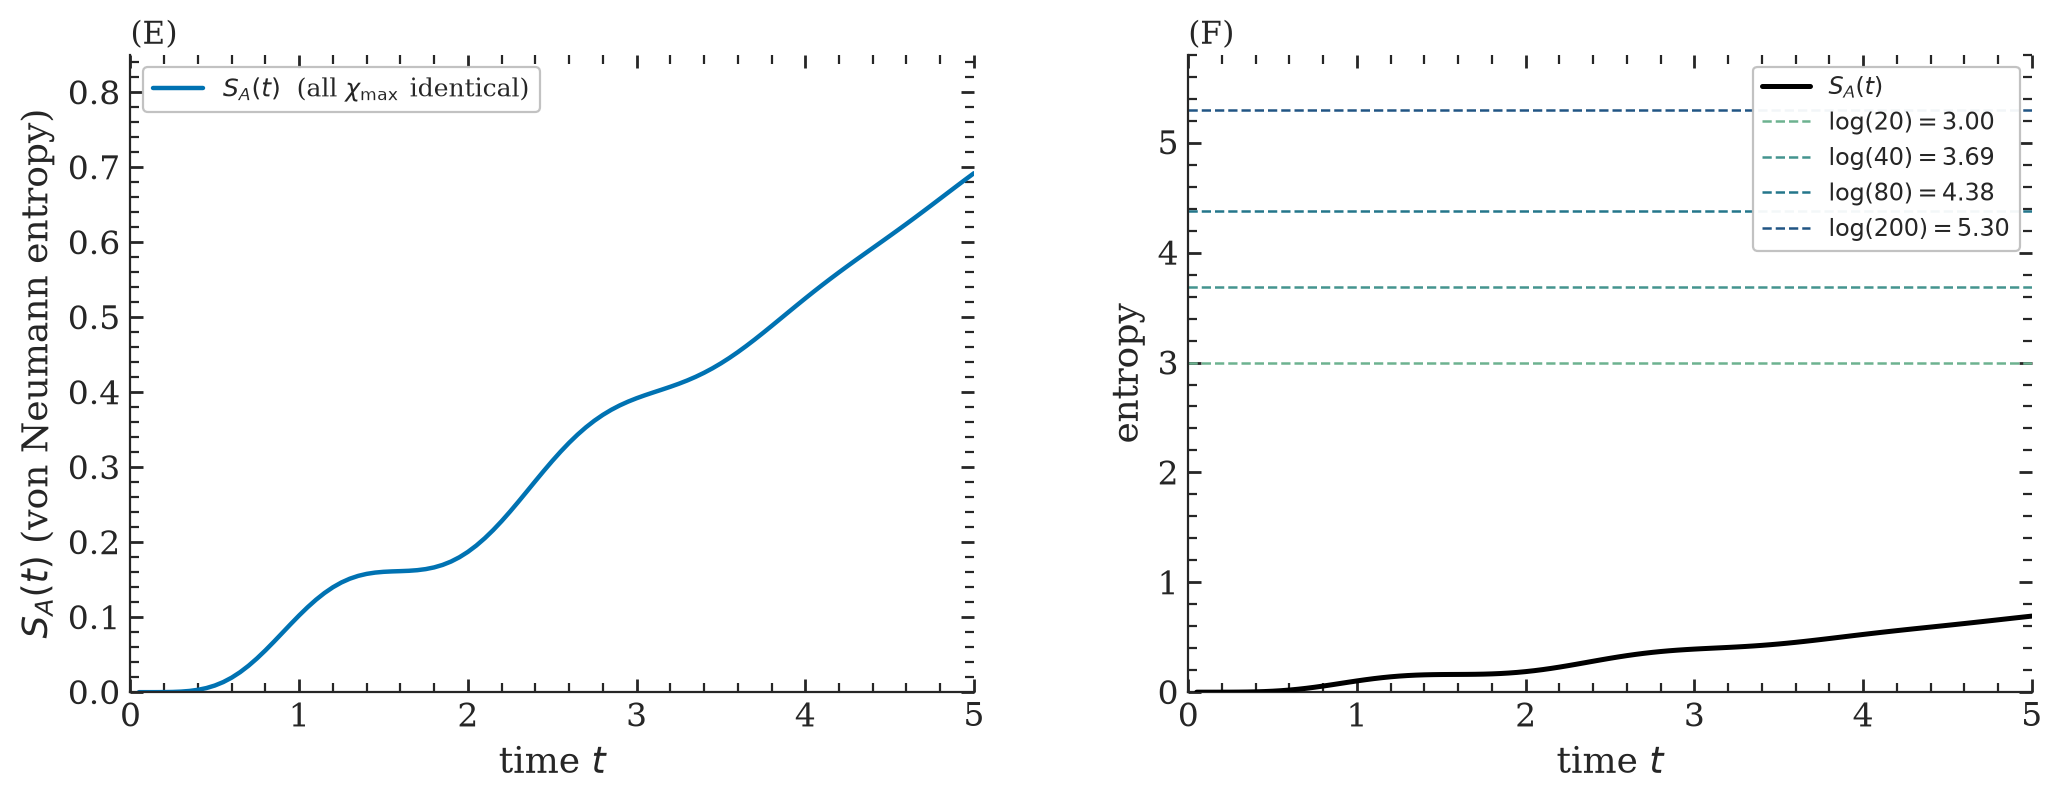
\includegraphics[width=\textwidth]{../results/figures/fig3_entropy.png}
  \caption{\textbf{(E)} Von Neumann entanglement entropy $S_A(t)$ for $h=2.0$.
    All $\chi_{\max}$ values give identical results, confirming convergence.
    \textbf{(F)} Same entropy (black) against the maximum representable entropy
    $\ln(\chi_{\max})$ for each bond dimension (dashed lines). Even at $t=5$,
    $S_A \approx 0.69 \ll \ln(20) \approx 3.0$: the simulation has large
    headroom before the bond dimension becomes a bottleneck.}
  \label{fig:entropy}
\end{figure}

Figure~\ref{fig:entropy} shows the entanglement entropy growth. For a generic
non-integrable model after a quench, $S_A(t) \sim t$ linearly, requiring
exponentially growing $\chi_{\max}$: the fundamental barrier to long-time TEBD
simulations. The TFIM instead shows $S_A \approx 0.69$ at $t=5$, far below any
$\ln(\chi_{\max})$ saturation limit. This is why all $\chi_{\max}$ from $20$ to
$200$ give identical $\lambda(t)$ results: the state is extremely compressible
throughout the simulation window.

\subsection{Cusp sharpness and bond dimension}

\begin{figure}[H]
  \centering
  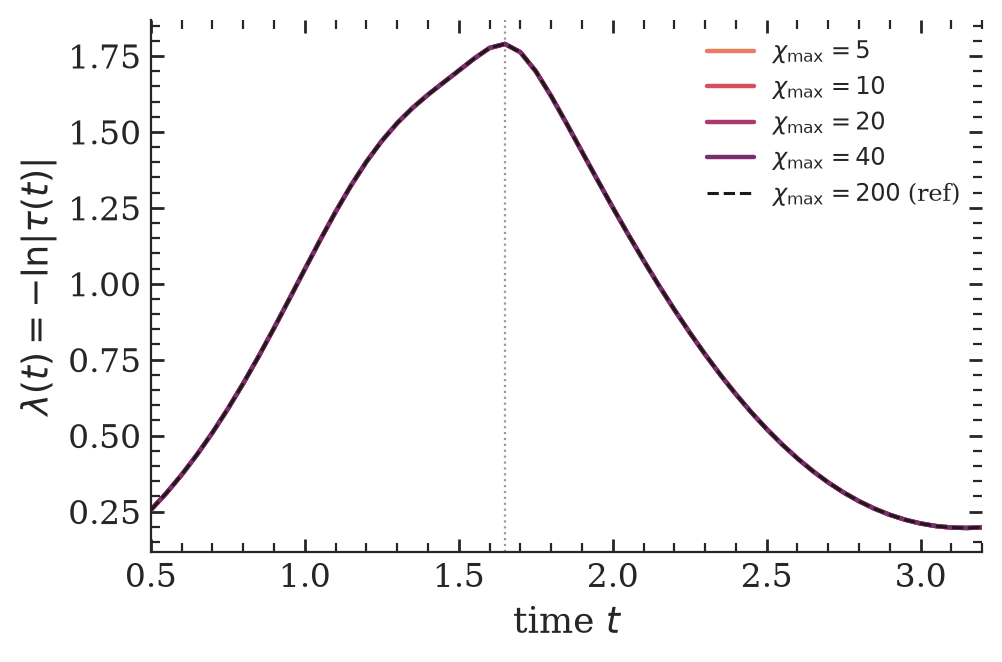
\includegraphics[width=0.72\textwidth]{../results/figures/fig5_cusp_sharpness.png}
  \caption{Rate function $\lambda(t)$ near the first cusp of $h=2.0$ for
    $\chi_{\max} \in \{5,10,20,40\}$ and reference $\chi_{\max}=200$ (dashed).
    All curves are indistinguishable to plotting precision, confirming that even
    $\chi_{\max}=5$ captures the DPT accurately. In a generic non-integrable
    model the lines would be expected to visibly separate, with smaller $\chi$
    rounding the cusp. The
    vertical dotted line marks $t^*_0 = 1.65$.}
  \label{fig:cusp}
\end{figure}

Figure~\ref{fig:cusp} makes the low-entanglement point concrete: even
$\chi_{\max}=5$ reproduces the cusp to within $10^{-9}$ of the converged
result at $t=1.65$ (verified against $\chi_{\max}=200$). At $t=1.65$, the system has built up only modest entanglement
($S_A \approx 0.18$), so all $\chi_{\max}$ values accurately represent the
state. The cusp rounding effect expected for small $\chi$ in a generic model
is completely absent here.

\subsection{Resolving $h=0.8$: DPT below the equilibrium critical field}
\label{sec:h08}

At $h=0.8$ (below the QPT at $h=1$), the $t\leq 5$ simulation shows a local
maximum in $\lambda(t)$ at $t\approx 4.6$, which is ambiguous at first glance:
it could be a genuine DPT or a broad smooth feature. An extended simulation to
$t=15$ with $\chi_{\max}=80$ reveals a second peak at $t\approx 14.9$ (compared
to the predicted $t^*_1 = 3\times 4.6 = 13.8$ for a DPT with period
$t^*=9.2$). The shift of $+1.1$ at late times is consistent with bond dimension
saturation at $t\approx 12$ ($\chi_A = 80$, trunc\_err $\approx 5\times10^{-9}$).
This is strong evidence for a genuine DPT. For the ferromagnetic ground-state
initial condition, the DPT threshold is exactly $h=1$ \cite{heyl2013}; our
result indicates that the DPT threshold for the Neel initial state is
$h_{\rm DPT} < 1$, an interesting distinction between the two quench protocols.

% ============================================================
\section{Conclusion}
% ============================================================

iTEBD was implemented from scratch in Python, cross-checked against the MATLAB
reference provided in the course notes, and used to study DPTs in the
infinite TFIM. The main findings are: (i) cusps in $\lambda(t)$ appear for $h>1$ with the
ferromagnetic ground-state initial condition \cite{heyl2013}, and for $h\geq
0.8$ with the Neel initial state (this work);
(ii) Trotter discretization dominates the error by six orders of magnitude over
bond-dimension truncation, a direct consequence of the TFIM's free-fermion
integrability; (iii) even $\chi_{\max}=5$ reproduces the DPT accurately,
showing the TFIM is far from the challenging regime where TEBD breaks down. The
iTEBD framework (infinite MPS, Vidal canonical form, Trotter gates, transfer
matrix) is a clean and powerful approach to non-equilibrium dynamics in 1D
quantum systems.

\begin{thebibliography}{9}

\bibitem{heyl2013}
M.~Heyl, A.~Polkovnikov, and S.~Kehrein,
\textit{Dynamical Quantum Phase Transitions in the Transverse-Field Ising Model},
Phys.~Rev.~Lett.~\textbf{110}, 135704 (2013).

\bibitem{vidal2007}
G.~Vidal,
\textit{Classical Simulation of Infinite-Size Quantum Lattice Systems in One Spatial Dimension},
Phys.~Rev.~Lett.~\textbf{98}, 070201 (2007).

\bibitem{suzuki1976}
M.~Suzuki,
\textit{Generalized Trotter's formula and systematic approximants of exponential operators and inner derivations with applications to many-body problems},
Commun.~Math.~Phys.~\textbf{51}, 183 (1976).

\bibitem{hatano2005}
N.~Hatano and M.~Suzuki,
\textit{Finding Exponential Product Formulas of Higher Orders},
in \textit{Quantum Annealing and Other Optimization Methods},
Springer Berlin Heidelberg, pp.~37--68 (2005).

\bibitem{sachdev2011}
S.~Sachdev,
\textit{Quantum Phase Transitions}, 2nd ed., Cambridge University Press (2011).

\end{thebibliography}

\end{document}
